\documentclass[american,ignorenonframetext,notheorems]{beamer}
\usetheme{Antibes}
\useinnertheme[shadow]{rounded}
\makeatletter
\defbeamertemplate*{headline}{subtree theme}
{%
    \begin{beamercolorbox}[wd=\paperwidth,colsep=1.5pt]{upper separation line head}
    \end{beamercolorbox}
    \begin{beamercolorbox}[wd=\paperwidth,ht=2.5ex,dp=1.125ex,%
      leftskip=.3cm,rightskip=.3cm plus1fil]{title in head/foot}
      \usebeamerfont{title in head/foot}\insertsectionnumber \hskip.5em \insertsectionhead
    \end{beamercolorbox}
    \begin{beamercolorbox}[wd=\paperwidth,ht=2.5ex,dp=1.125ex,%
      leftskip=.3cm,rightskip=.3cm plus1fil]{section in head/foot}
      \usebeamerfont{section in head/foot}%
      \ifbeamer@tree@showhooks
        \setbox\beamer@tempbox=\hbox{\insertsubsectionhead}%
        \ifdim\wd\beamer@tempbox>1pt%
          \hskip2pt\raise1.9pt\hbox{\vrule width0.4pt height1.875ex\vrule width 5pt height0.4pt}%
          \hskip1pt%
        \fi%
      \else%  
        \hskip6pt%
      \fi%
      \insertsubsectionhead
    \end{beamercolorbox}
    \begin{beamercolorbox}[wd=\paperwidth,ht=2.5ex,dp=1.125ex,%
      leftskip=.3cm,rightskip=.3cm plus1fil]{subsection in head/foot}
      \usebeamerfont{subsection in head/foot}%
      \ifbeamer@tree@showhooks
        \setbox\beamer@tempbox=\hbox{\insertsubsubsectionhead}%
        \ifdim\wd\beamer@tempbox>1pt%
          \hskip9.4pt\raise1.9pt\hbox{\vrule width0.4pt height1.875ex\vrule width 5pt height0.4pt}%
          \hskip1pt%
        \fi%
      \else%  
        \hskip12pt%
      \fi%
      \insertsubsubsectionhead
    \end{beamercolorbox}
    \begin{beamercolorbox}[wd=\paperwidth,colsep=1.5pt]{lower separation line head}
    \end{beamercolorbox}
}
\makeatother
\usecolortheme{iwr}
\usepackage{../mathsim}
\tikzset{velox/.style={color=black,draw,fill=red,thick,%
    shape=diamond,aspect=.4,
    inner sep=1.3pt,transform shape}}
\tikzset{veloy/.style={color=black,draw,fill=red,thick,%
    shape=diamond,aspect=2.5,
    inner sep=1.3pt,transform shape}}
\tikzset{veloxy/.style={color=black,draw,fill=red,thick,%
    shape=star,star points=4,star point ratio=2.2,
    inner sep=1.3pt,transform shape}}
\tikzset{pressure/.style={color=black,draw,fill=cyan,thick,%
    shape=circle,inner sep=2pt,transform shape}}
\tikzset{velo/.style={transform shape,double=red,arrows={-Stealth[open,fill=red]}}}

%% Macros for drawing degrees of freedom for different shapes/elements.
%% Arguments are always:
%%   #1: Starting point
%%   #2: End point
%%   #3: polynomial degree
%%   #4: node settings

\tikzset{pics/edgenormal/.style args={#1/#2/#3/#4}{%
    code={%
      \draw #1 -- #2
      node foreach \x [evaluate=\x as \xval] in {1,...,#3} [#4,sloped,pos=\xval/(#3+1)] {};
      }
}}


%% Macros for drawing degrees of freedom for different shapes/elements.
%% Arguments are always:
%%   #1: polynomial degree
%%   #2: node settings

\tikzset{pics/tripile/.style args={#1/#2}{%
    code={%
      \coordinate (top) at (0,#1);
      \foreach \i in{0,...,#1}
      \foreach \j in{0,...,\i}
      {
        \tikzmath{
          \y = .3*(2/3*#1-\i)*cos(30);
          \x = .3*(\i/2-\j);
        }
        \node[#2] at (\x,\y) {};
      }
    }
}}

\tikzset{pics/tensor/.style args={#1/#2/#3}{%
    code={%
      \coordinate (top) at (0,#1);
      \foreach \i in{0,...,#1}
      \foreach \j in{0,...,#2}
      {
        \tikzmath{
          \y = 2*(\i+1)/(#1+2);
          \x = 2*(\j+1)/(#2+2);
        }
        \node[#3] at (\x,\y) {};
      }
    }
}}

\tikzset{pics/pfem/.style args={#1/#2}{%
    code={%
      \tikzmath{ \ytop=2*cos(30); }
      \coordinate (top) at (0,\ytop);

      \foreach \i in{0,...,#1}
      \foreach \j in{0,...,\i}
      {
        \tikzmath{
          \y = \ytop-\ytop*\i/#1;
          \x = 2*(\i/2-\j)/#1+1;
        }
        \node[#2] at (\x,\y) {};
      }
    }
}}

\tikzset{pics/qfem/.style args={#1/#2}{%
    code={%
      \foreach \i in{0,...,#1}
      \foreach \j in{0,...,#1}
      {
        \tikzmath{
          \y = 2-2*\i/#1;
          \x = 2-2*\j/#1;
        }
        \node[#2] at (\x,\y) {};
      }
    }
}}

%%% Local Variables:
%%% mode: latex
%%% TeX-master: "all"
%%% End:

\mathtoolsset{showonlyrefs}
\excludecomment{solution}
\externaldocument{main}

\makeatletter
\def\blocktheorem#1#2(#3){\begin{block}{#3 \capitalizewords{#1}%
      \def\tmp{#2}\ifx\tmp\empty{}\else (#2)\fi}}
\def\endblocktheorem{\end{block}}
\makeatother
\def\mylabel#1{}
\let\label\mylabel
%\renewcommand{\label}[1]{}
\renewcommand{\eqref}[1]{(\ref{#1})}
\renewcommand{\define}[1]{\textbf{#1}}
\begin{document}
\section{Introduction: from elliptic to mixed problems}
\subsection{Elliptic systems: linear elasticity}
\subsubsection{Example: weak form of the Lamé-Navier equations}
\subsubsection{The finite element toolbox}
\subsubsection{Where things go wrong}

\begin{frame}
  \frametitle{Example: hanging sheet}
  \begin{itemize}
  \item $\domain = (-1,1)^2$
  \item $\vf = (0,-1)^T$
  \item $\vu = 0$ at $(x,1)$
  \item $\strain u \n = 0$ on remaining boundary
  \item $\mu=1$ and $\lambda$ varies
  \item Two different finite element methods
    \begin{itemize}
    \item Red: bilinear elements
    \item Blue: Hdiv-DG (later in this class)
    \end{itemize}
  \end{itemize}
\end{frame}

\begin{frame}
  \frametitle{Example: hanging sheet}
  \centering
  \begin{tabular}{cc}
    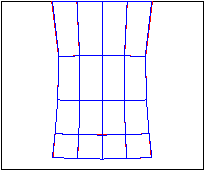
\includegraphics[width=.45\textwidth]{./graph/elasticity/stalactite-0}
    &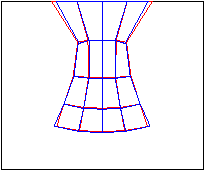
\includegraphics[width=.45\textwidth]{./graph/elasticity/stalactite-1}
    \\
    $\lambda = 1$&$\lambda = 10$
  \end{tabular}
\end{frame}

\begin{frame}
  \frametitle{Example: hanging sheet}
  \centering
  \begin{tabular}{ccc}
    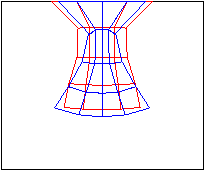
\includegraphics[width=.45\textwidth]{./graph/elasticity/stalactite-2}
    &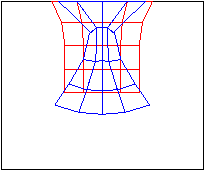
\includegraphics[width=.45\textwidth]{./graph/elasticity/stalactite-3}
    \\
    $\lambda = 100$&$\lambda = 1000$
  \end{tabular}
\end{frame}

\begin{frame}
  \frametitle{Example: hanging sheet}
  \centering
  \begin{tabular}{ccc}
    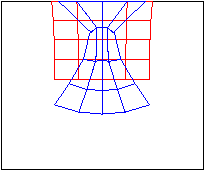
\includegraphics[width=.45\textwidth]{./graph/elasticity/stalactite-4}
    &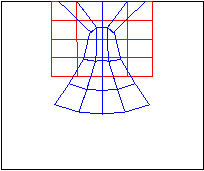
\includegraphics[width=.45\textwidth]{./graph/elasticity/stalactite-5}
    \\
    $\lambda = 10000$&$\lambda = 100000$
  \end{tabular}
\end{frame}

\begin{frame}
  \frametitle{Example: hanging sheet}
  \centering
  \begin{tabular}{ccc}
    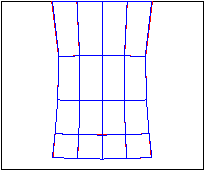
\includegraphics[width=.45\textwidth]{./graph/elasticity/stalactite-0}
    &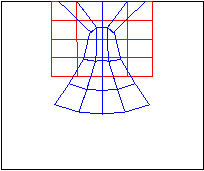
\includegraphics[width=.45\textwidth]{./graph/elasticity/stalactite-5}
    \\
    $\lambda = 1$&$\lambda = 100000$
  \end{tabular}
\end{frame}

\begin{frame}
  \frametitle{Manufactured setting}
  \begin{itemize}
  \item $\domain = (-1,1)^2$
  \item $\vu = 0$ on $\d\domain$
  \item Right hand side computed from known solution
  \item $\mu=1$ and $\lambda$ varies
  \end{itemize}
\end{frame}

\begin{frame}
  \frametitle{Errors for a manufactured setting}
  \centering
  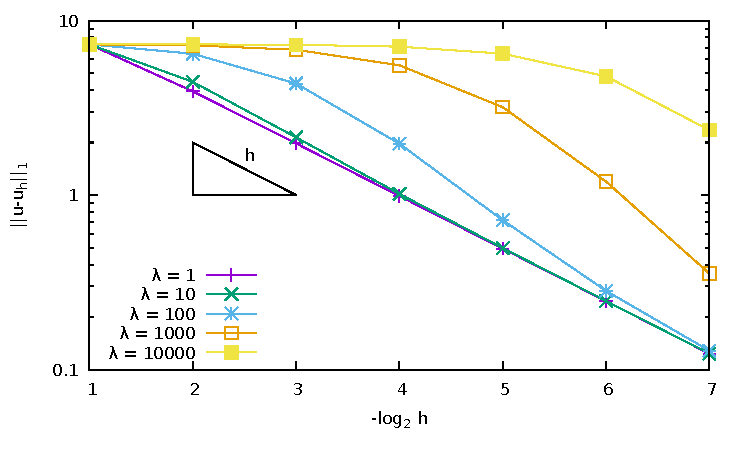
\includegraphics[width=.8\textwidth]{./graph/elasticity/locking}
\end{frame}

\subsubsection{A mixed formulation}
\begin{frame}
  \frametitle{Avoiding large parameters}

  \begin{gather}
    a(\vu,\vv) \equiv 2\mu\form(\strain \vu, \strain \vv)
    + \lambda \form(\div \vu, \div \vv)
    = \form(\vf,\vv)
  \end{gather}
\end{frame}

\subsection{Abstract saddle-point systems}

\begin{frame}
  \frametitle{Example: one-dimensional $P_1-P_1$ elements}
  \begin{center}
      \includegraphics[width=.7\textwidth]{./fig/p1-p1-1d}
  \end{center}
\end{frame}

\begin{frame}
  \frametitle{Small patches with Dirichlet boundary}
  \begin{center}
    \hfill
    \includegraphics[width=.3\textwidth]{./fig/patch1.tikz}
    \hfill
    \includegraphics[width=.3\textwidth]{./fig/patch2.tikz}
    \hfill\mbox{}
  \end{center}
\end{frame}

\begin{frame}
  \frametitle{Checkerboard modes}
  
\end{frame}

\subsection{MINI element}

\begin{frame}
  \frametitle{The $P_1$ element in barycentric coordinates}
  \begin{columns}
    \begin{column}{.5\textwidth}
      \begin{center}
        \includegraphics[width=.6\textwidth]{./fig/p1-p.tikz}
      \end{center}
    \end{column}
    \begin{column}{.5\textwidth}
      \begin{gather}
        \phi_i = \lambda_i,
        \quad i=0,1,2
      \end{gather}
    \end{column}
  \end{columns}
\end{frame}

\begin{frame}
  \frametitle{The $P_2$ element in barycentric coordinates}
  \begin{columns}
    \begin{column}{.5\textwidth}
      \begin{center}
        \includegraphics[width=.6\textwidth]{./fig/p2-p.tikz}
      \end{center}
    \end{column}
    \begin{column}{.5\textwidth}
      \begin{xalignat*}2
        \phi_{ii} &= 2\lambda_i^2 - \lambda_i,
        &i&=0,1,2\\
        \phi_{ij} &= 4\lambda_i\lambda_j
        &j&\neq i
      \end{xalignat*}
    \end{column}
  \end{columns}
\end{frame}

\begin{frame}
  \frametitle{The $P_3$ element in barycentric coordinates}
  \begin{columns}
    \begin{column}{.5\textwidth}
      \begin{center}
        \includegraphics[width=.6\textwidth]{./fig/p3-p.tikz}
      \end{center}
    \end{column}
    \begin{column}{.5\textwidth}
      \begin{xalignat*}2
        \phi_{iii} &= \tfrac12 \lambda_i(3\lambda_i-1)(3\lambda_i-2)
        &i&=0,1,2\\
        \phi_{ij} &= \tfrac92\lambda_i\lambda_j(3\lambda_j-1)
        &j&\neq i\\
        \phi_0 &= 27\lambda_0\lambda_1\lambda_2
      \end{xalignat*}
    \end{column}
  \end{columns}
\end{frame}

\end{document}

%%% Local Variables:
%%% mode: latex
%%% TeX-master: t
%%% End:
